\documentclass[times, utf8, diplomski]{fer}
\usepackage{booktabs}
\usepackage{pdfpages}
\usepackage{catchfile}
\usepackage{xparse}
\usepackage{listings}

% environment setup
\ExplSyntaxOn
\NewDocumentCommand{\getenv}{om}
 {
  \sys_get_shell:nnN { kpsewhich ~ --var-value ~ #2 } { } \l_tmpa_tl
  \tl_trim_spaces:N \l_tmpa_tl
  \IfNoValueTF { #1 }
   {
    \tl_use:N \l_tmpa_tl
   }
   {
    \tl_set_eq:NN #1 \l_tmpa_tl
   }
 }
\ExplSyntaxOff

\getenv[\resdir]{THESIS_RESDIR}
% done

\begin{document}
\thesisnumber{2568}

\title{Design of a strongly-typed programming language}

\author{Petar Mihalj}

\maketitle

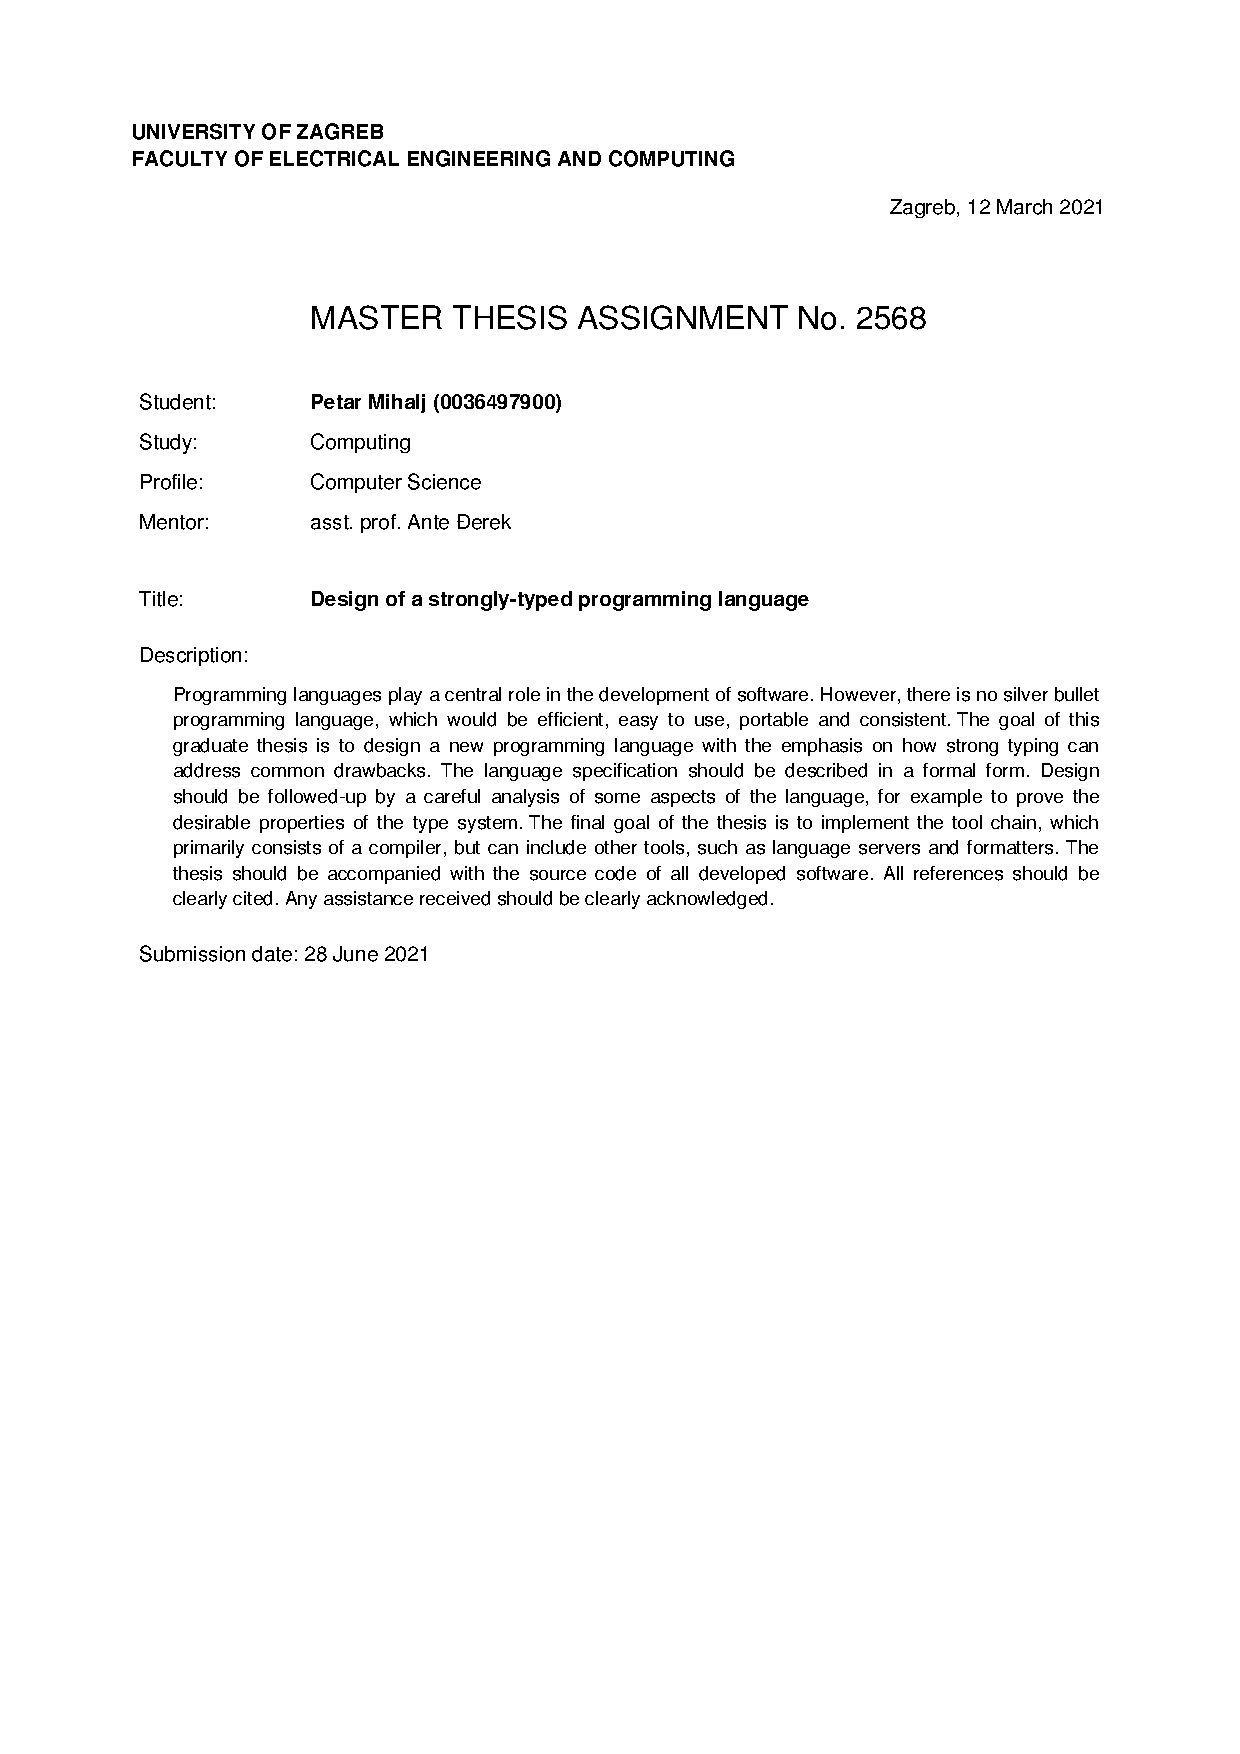
\includepdf[pages={1,2}]{\resdir/task.pdf}

\zahvala{I thank everybody...}

\tableofcontents

\chapter{Introduction}

The programming language developed as a part of this thesis is called AGT.
The name AGT stands for an unfortunate fact that the names of all precious stones
are taken by other programming languages, hence "All Gems are Taken".

AGT is a statically and strongly typed language, with a highly expressive type system.
The type system is used for three main purposes:

\begin{enumerate}
    \item types determine the size of values in memory
    \item types enable polymorphic behaviour (of both builtin and user-defined (struct) types)
    \item types allow for compile-time computation
\end{enumerate}

The language also allows for implementation of object lifetime constructs, 
such as those seen in languages like C++ or Rust; object creation, copying and destruction.
These constructs can be used to implement various object ownership semantics, 
which will be demonstrated in later chapters.

The reference AGT compiler (AGTC) produces executable binaries only.
This is in sharp contrast to some other languages, which can produce object files, 
to later be linked into executables for a particular runtime, 
or used to augument the runtime environment itself (kernel modules, for example). 
This decision was made primarely because the goal of the thesis was to study the language 
from the application programmers perspective. 
This goal implies that AGT is running on a rich runtime environement, 
where heap memory management and standard I/O are available.
Future updates to AGT specification are meant to allow AGT to be compiled
into linkable files compatible with various platform specific ABIs.

The compiler frontend is implemented using Python3 programming language,
while the backend uses LLVM \citep{c_llvm_lattner} compiler infrastructure.
Allowing for some simplification, AGT is first compiled into LLVM intermediate representation (LLVM-IR),
and than is turned into executable by a chain of tools for compiling LLVM-IR and 
linking the resultuing object files into executables.

\section{Paper organization}

This master thesis will gradually introduce the reader to AGT, starting from the simplified introduction
to syntax and semantics, with an emphasis on type system and inference. This introduction will be
augumented with simple examples of AGT code. 

After the surface-level exploration of the language, we will study the language in depth. 
This part will have many references to the AGTC reference implementation, 
rather than to a separate formal specification. Since AGT is still not a finalized product,
formal specification does not exist, and it's functionality is determined by a reference compiler.
We will mostly focus on the type system, since it is unorthodox and is the main contribution of the author.
In this part, the author will justify the decisions which have been made on all levels of AGT design process.

In the last part, we will address the issues AGT has both on definition and implementation levels,
and comment on the various features that can be improved or added to the language.

\chapter{The AGT Programming Language - a gentle introduction}

Before diving into

\section{Hello world!}

Let us first check out an example AGT program:

\lstinputlisting[basicstyle=\small, numbers=left]{\resdir/programs/intro.agt}

Every AGT program has to have a function called main, which returns a 32-bit-wide integer.
Some functions, like \texttt{outnl}, don't return anything. It is important to note that you can't
specify that a function returns \texttt{void} like in C for example.

A \texttt{let <x> = <y>;} construct is \textit{initialization assignment} statement.
This roughly translates to an allocation of memory on a stack (which is allocated at the newly
generated \textit{location} of <x>), and copying the value of expression <y>
to the location of identifier <x>.

Note that call of the function \texttt{in} is \textit{parametrized} by a \textit{type argument} \texttt{i32}.
Type arguments are in contrast to the \textit{value arguments}, which carry value too, along with a type.
The function \texttt{in} is a builtin, and the \texttt{i32} is used to signal the compiler
that we want an instance of this function which returns an \texttt{i32}, 
rather than a \texttt{char}, for example. 
Of course, user-defined functions can also have \textit{type parameters}, along with \textit{value parameters};
we will get to these later.

Notice that we used the \texttt{cast<i32>} builtin function to convert \texttt{b} to \texttt{i32}
before passing it to function \texttt{mul}. If we didn't do that, the compiler would signal that it can't
compute the expression \texttt{a*b}, since multiplication is predefined only for integer types of same size.
Apart from the \texttt{i8} and \texttt{i32} we used in this example, \texttt{i16} and \texttt{i32} are also
available.

There is a certain feature that you might have missed while inspecting the code; namely the abscence of
types in the definition of function \texttt{mul}.
While some \texttt{dynamically typed} languages (ex. Python) allow for object of any type to be passsed
to the function, AGT behaves quite differently. 

Every time AGTC (AGT compiler) encounters a function call,
it tries to infer a \textit{function type}. Function type is inferred from function definitions. 
Consequently, you can think of the definitions in source code more as \texttt{templates} for synthesis
of actual code, than the actual representation of code. 
These definitions lack types, and can't be considered in isolation.
In this example, the call of function \texttt{mul} causes the compiler to try to infer a function type.

It is important to emphasize that one function definition can be a source of many function types.
The \texttt{outnl} (output with newline) function is a prime example of this behaviour.
It is called three times, with argument of types \texttt{i32}, \texttt{i8} and \texttt{i32}.
Thus, the compiler has to infer two function types, 
one which can be fed with an \texttt{i8}, and one with \texttt{i32}.
The success of this inference corresponds with compilers ability to infer function body of
the given function definition.
This will be possible if and only if the compiler can also infer the function type \texttt{out} 
function which can take ...
The property of \texttt{outnl} function definition which allows it to be a source for inference
of two distinct function types, given that it \textit{makes sense} for these types 
(regarding the function body), is called \bf{parametric polymorphism}.








\chapter{Conclusion}
Zaključak.

\bibliographystyle{dinat}
\bibliography{literatura}

\begin{sazetak}
Sažetak na hrvatskom jeziku.

\kljucnerijeci{Ključne riječi, odvojene zarezima.}
\end{sazetak}

% TODO: Navedite naslov na engleskom jeziku.
\engtitle{Title}
\begin{abstract}
Abstract.

\keywords{Keywords.}
\end{abstract}

\end{document}
